\section{Querying data from the PCDB}\label{sec_query_from_the_PCDB}

As figure \ref{fig_pgadmin3_inside_PCDB} shows, there are multiple schemas inside the PCDB. (Read about schemas in the \texttt{PostgreSQL} documentatin, \url{https://www.postgresql.org/docs/9.1/static/ddl-schemas.html})
The organization of the schemas in the PCDB is desribed in chapter \ref{chap_programming_the_PCDB}.

To browse a schema, simply select it with a doubl-click in the `Object browser.'
Selection by double-click will drop-down the objects inside the given schema, as shown in figure \ref{fig_pgadmin3_inside_config_data} for the \texttt{config\_data} schema inside the PCDB.

\begin{figure}[ht!]
\centering
  \begin{subfigure}{.45\textwidth}
  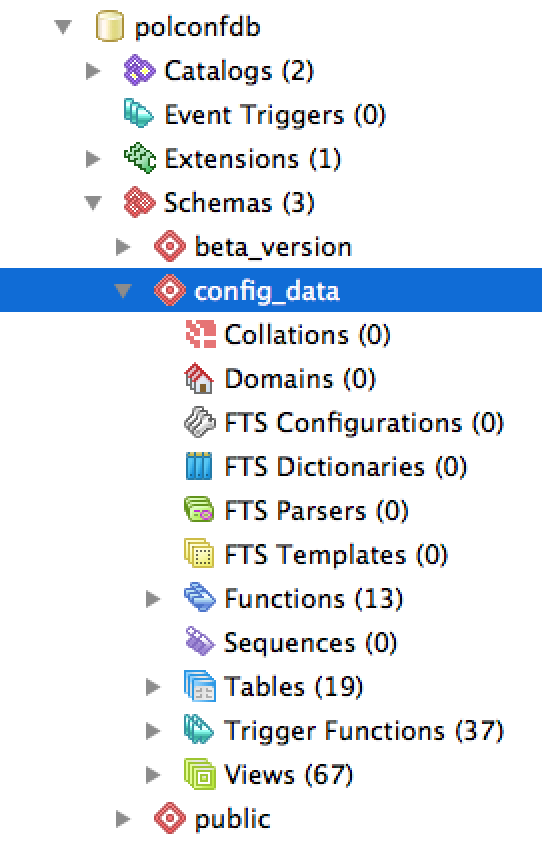
\includegraphics[width=\textwidth,trim= 0 0 0 0, clip]{pcdb_documentation_screenshots/pgadmin3_inside_config_data.png}
    \subcaption{View of `Object browser' window after selecting the \texttt{config\_data} schema of the \texttt{polconfdb} database in \texttt{pgAdmin3}.}
    \label{fig_pgadmin3_inside_config_data}
  \end{subfigure}
  ~%
  \begin{subfigure}{.45\textwidth}
  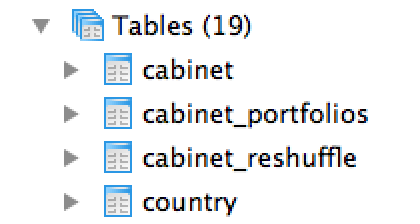
\includegraphics[width=\textwidth,trim= 0 0 0 0, clip]{pcdb_documentation_screenshots/pgadmin3_tables_inside_config_data.png}
    \subcaption{View of `Object browser' window after selecting tables in the \texttt{config\_data} schema of the \texttt{polconfdb} database in \texttt{pgAdmin3}.}
    \label{fig_pgadmin3_tables_inside_config_data}
  \end{subfigure} 
  \caption{Inside the \texttt{config\_data} schema of the \texttt{polconfdb} database in \texttt{pgAdmin3}.}
\end{figure}

There are a some contents you will usually be less concerned with, such as `Collations,' `Domains,' `FTS' objects, and `Sequences.' (Note that they are empty, as indicated by the zero in brackets after their names.)
Most important to you, in case you want to query data from the PCDB, are the `Tables' and `Views' objects.\footnote{
Tables are the permanent repositories that store the data of the PCDB; views are virtual tables based on the result-sets of pre-defined SQL-queries (queries are always executed when you query a view). Detailed descriptions of the content and definition of the tables and view in the PCDB are provided in chapter \ref{chap_programming_the_PCDB}.}
When you double-click on the `Tables' object in \texttt{pgAdmin3}'s `Object browser', a list of all tables in the current schema (here \texttt{config\_data}) will be displayed (see figure \ref{fig_pgadmin3_tables_inside_config_data}).

Double-clicking again on a particular table object will cause some changes in the tool bar: When selecting a particular table, the `Data Viewer' tool is activated (the icon that looks like a data table; right to the `SQL'-labeled magnifying glass, which is \texttt{pgAdmin3}'s built-in SQL-query editor).
The visual difference is shown in figures \ref{fig_pgadmin3_select_tables_toolbar} and \ref{fig_pgadmin3_select_a_table_toolbar}: 
When no particular table or view is selected, the `Data Viewer' icon is blured and not click-able (see figure \ref{fig_pgadmin3_select_tables_toolbar}); after selecting a particular table or view, you can double-click on the data viewer tool, and a data table window will pop up on your desktop.

\begin{figure}[ht!]
\centering
  \begin{subfigure}{.45\textwidth}
  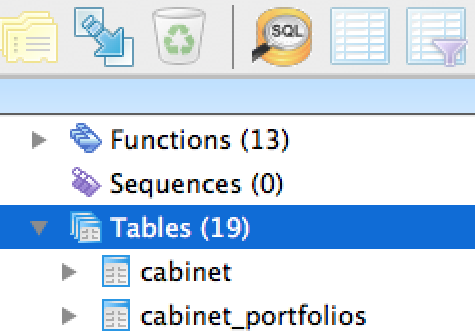
\includegraphics[width=\textwidth,trim= 0 0 0 0, clip]{pcdb_documentation_screenshots/pgadmin3_select_tables_toolbar.png}
    \subcaption{Tool bar when selecting `Tables' object in `Object browser' window.}
    \label{fig_pgadmin3_select_tables_toolbar}
  \end{subfigure}
  ~%
  \begin{subfigure}{.45\textwidth}
  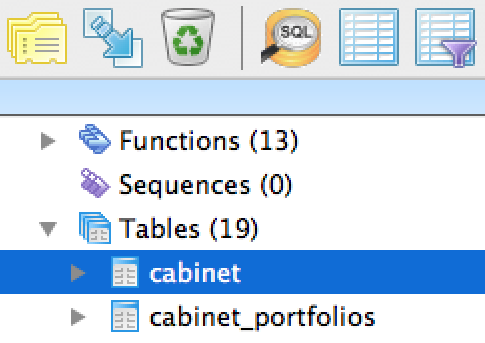
\includegraphics[width=\textwidth,trim= 0 0 0 0, clip]{pcdb_documentation_screenshots/pgadmin3_select_a_table_toolbar.png}
    \subcaption{Tool bar when selecting a particular table in `Object browser' window.}
    \label{fig_pgadmin3_select_a_table_toolbar}
  \end{subfigure} 
  \caption{Change in \texttt{pgAdmin3}'s tool bar when selecting a particular table.}
\end{figure}

  \subsection{Browse data in the PCDB: The `Data viewer' window}\label{subsec_data_viewer} 
Figure \ref{fig_pgadmin3_data_viewer_country} displayes the window that pops-up when selecting the country table in the \texttt{config\_data} schema in of the \texttt{polconfdb} database on the CMS database server.

\begin{figure}[ht!]
\centering
  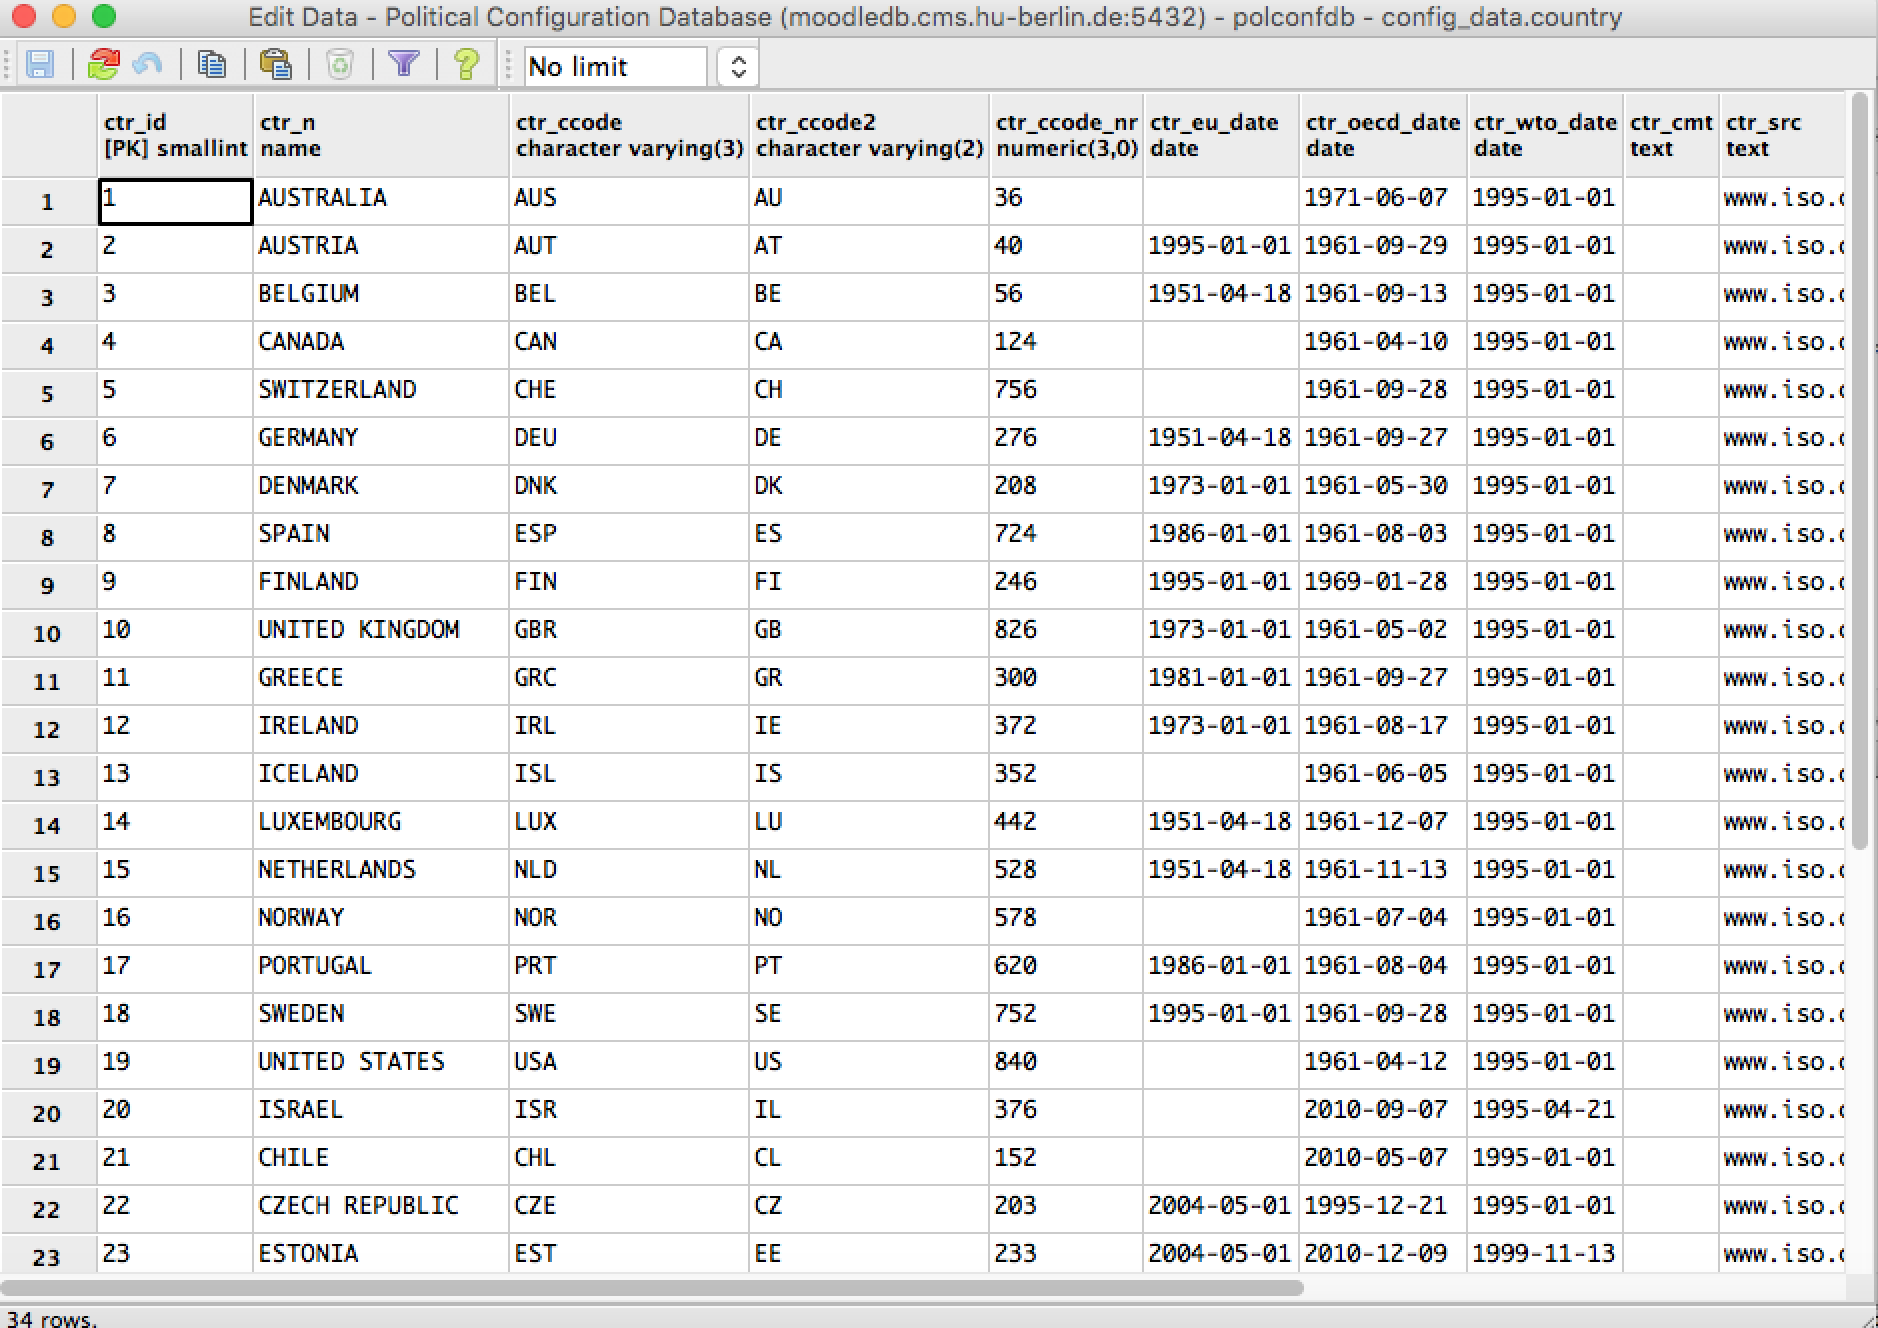
\includegraphics[width=.8\textwidth,trim= 0 0 0 0, clip]{pcdb_documentation_screenshots/pgadmin3_data_viewer_country.png}
    \caption{Data Viewer pop-up window of country table in \texttt{config\_data} schema.}
    \label{fig_pgadmin3_data_viewer_country}
\end{figure}

The `Data viewer' window has the following elements (from top to bottom):
\begin{itemize}
\item[-] The {\bf window header} informs you that this is an editor (i.e., if writing-rights are granted to your role, you can edit the data by double-clicking inside cells and change their content), and about the name of the server you are connected to (here ``Political Configuration Database''), the host and port number (``(moodledb.cms.hu-berlin.de:5432)''), as well as the database (``polconfdb''), and schema and table names (``config\_data.country''). This is in fact the all information you need to know which data table is displayed.

\item[-] The window's {\bf tool bar} allows you to refresh the current data table (icon with one red and one green circular arrow); and, in case you have writing rights, to save changes (blue shaded disc icon), or undo changes to the data (right-to-left upward-bend blue shaded arrow). 

\item[-] The {\bf main panel} displays the data of the selected table or view. 
Columns are variables, where the main panel's header displays variable names and types (e.g., \texttt{ctr\_id} and \texttt{smallint}), and contraints are displayed in square brackets (e.g., \texttt{[PK]}, which stands for primary key).
By default, all rows are listed; but you can limit the number of rows displayed in the most-right tool bar panel by typing a number in the input window label `No limit' by default.) 

\item[-] The {\bf window footer} informs you how many rows the displayed data has.
\end{itemize}

  \subsection{Export data from the PCDB: The SQL-query tool}\label{subsec_sql_query_tool}
While the `Data Viewer' only allows to view data (and to edit data only manually, one-by-one, in case you have writing-rights), \texttt{pgAdmin3}'s SQL-query tool allows to actually write and execute SQL-queries to obtain data from tables and views. 
Moreover, the SQL-Query tool allows to export the result-set of your query (a data table) to a file. 
Using the SQL-query tool is therefore the easiest way to export data from the PCDB.

Figure \ref{fig_pgadmin3_sql_query_tool_editor_country} and \ref{fig_pgadmin3_sql_query_tool_builder_country} show the two ways in which you may query data using the SQL-query tool, again using the example of of the country table in the \texttt{config\_data} schema.
\begin{itemize}
\item[(a)]{You may explicitly write SQL code to define a query in the `SQL Editor' tab of the SQL-query tool window's top panel. Double-clicking the green play-button in the SQL-query tool's toolbar (second from left in figure \ref{fig_pgadmin3_sql_query_tool_toolbar}) will execute the query; the result will be displayed as data table in the `Output pane' (bottom panel of the window).}
\item[(b)]{You may construct your query manually, using the in the `Graphical Query Builder' tab of the SQL-query tool window's top panel. Double-clicking the green play-button in the SQL-query tool's toolbar (second from left in figure \ref{fig_pgadmin3_sql_query_tool_toolbar}) will return the manually built query in explicit SQL code, execute it, and display the result as data table in the `Output pane' (bottom panel of the window).}
\end{itemize}

\begin{figure}[ht!]
\centering
  \begin{subfigure}{.45\textwidth}
  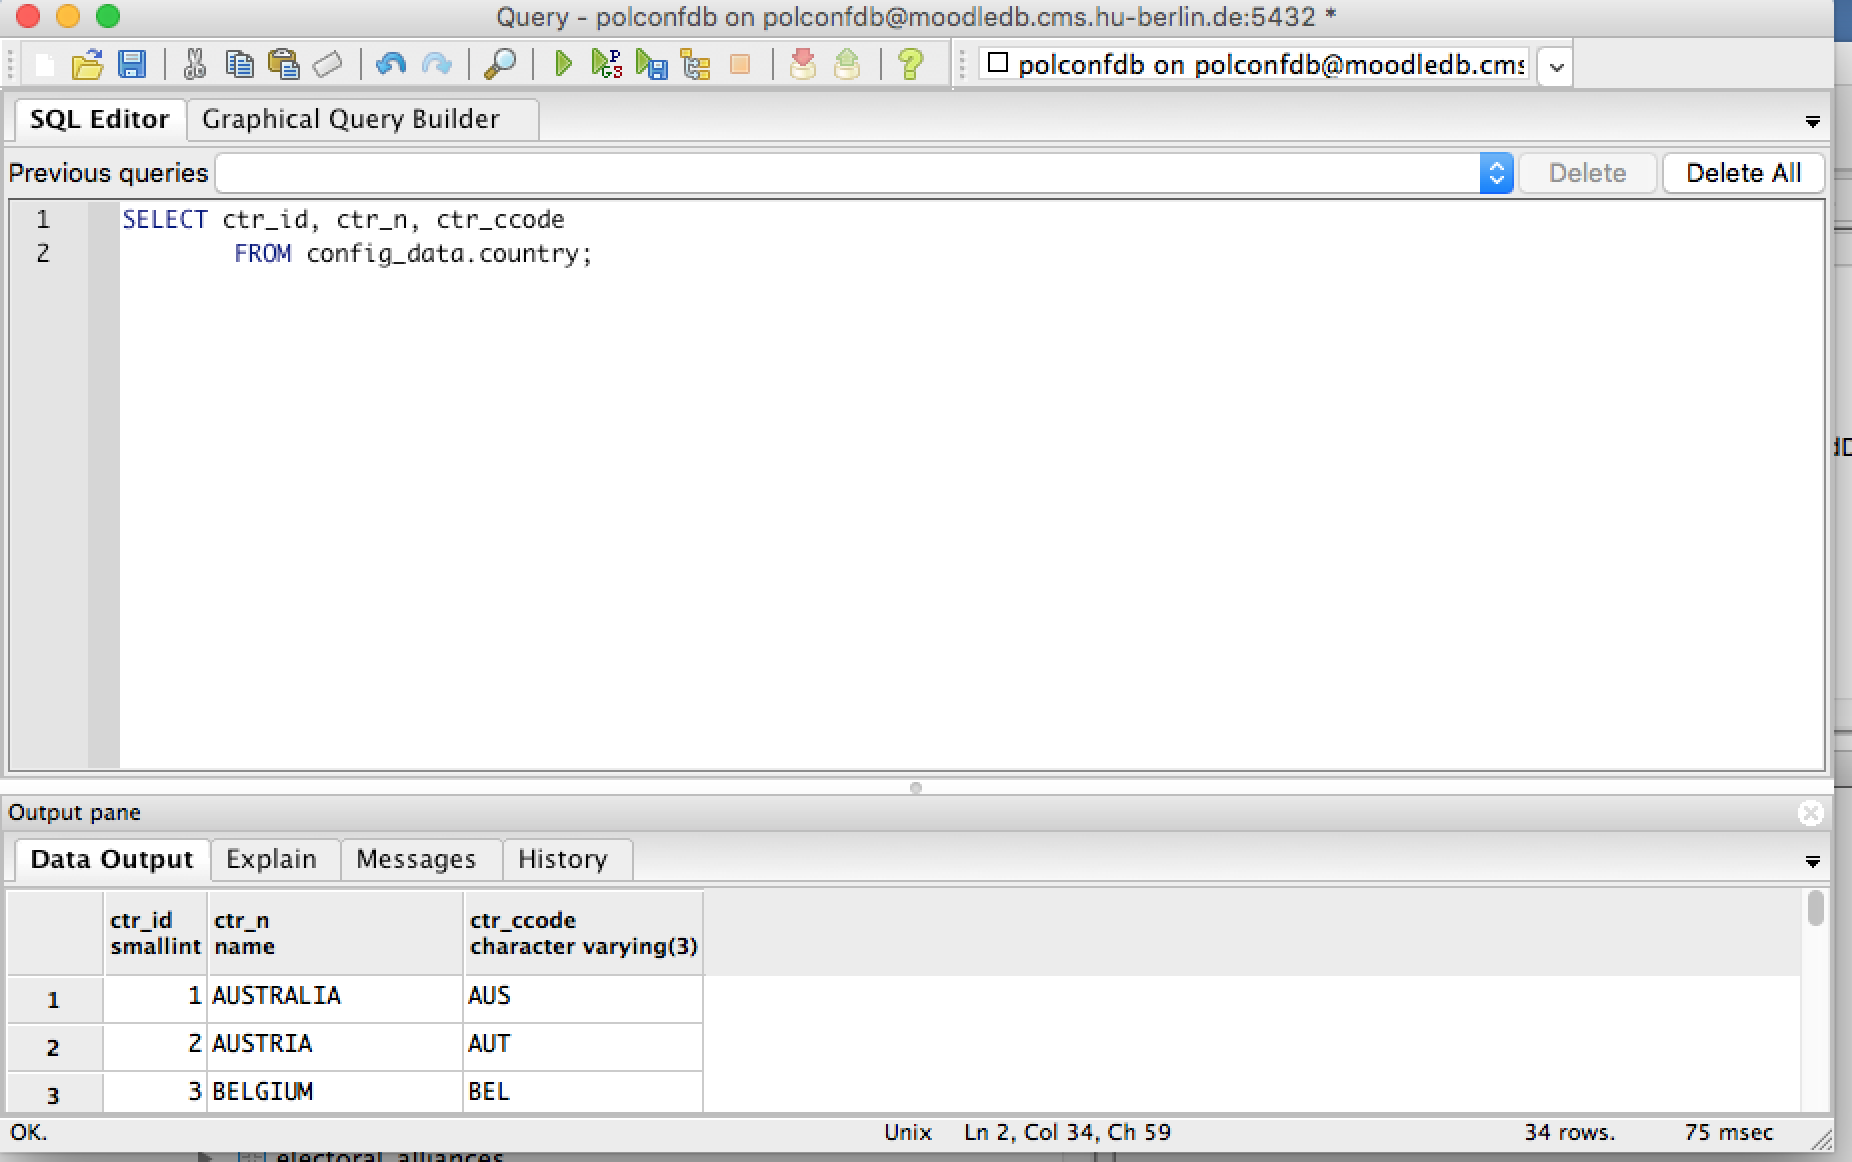
\includegraphics[width=\textwidth,trim= 0 0 0 0, clip]{pcdb_documentation_screenshots/pgadmin3_sql_query_tool_editor_country.png}
    \subcaption{Query data with explicit SQL code from country table in the `SQL Editor' tab.}
    \label{fig_pgadmin3_sql_query_tool_editor_country}
  \end{subfigure}
  ~%
  \begin{subfigure}{.45\textwidth}
  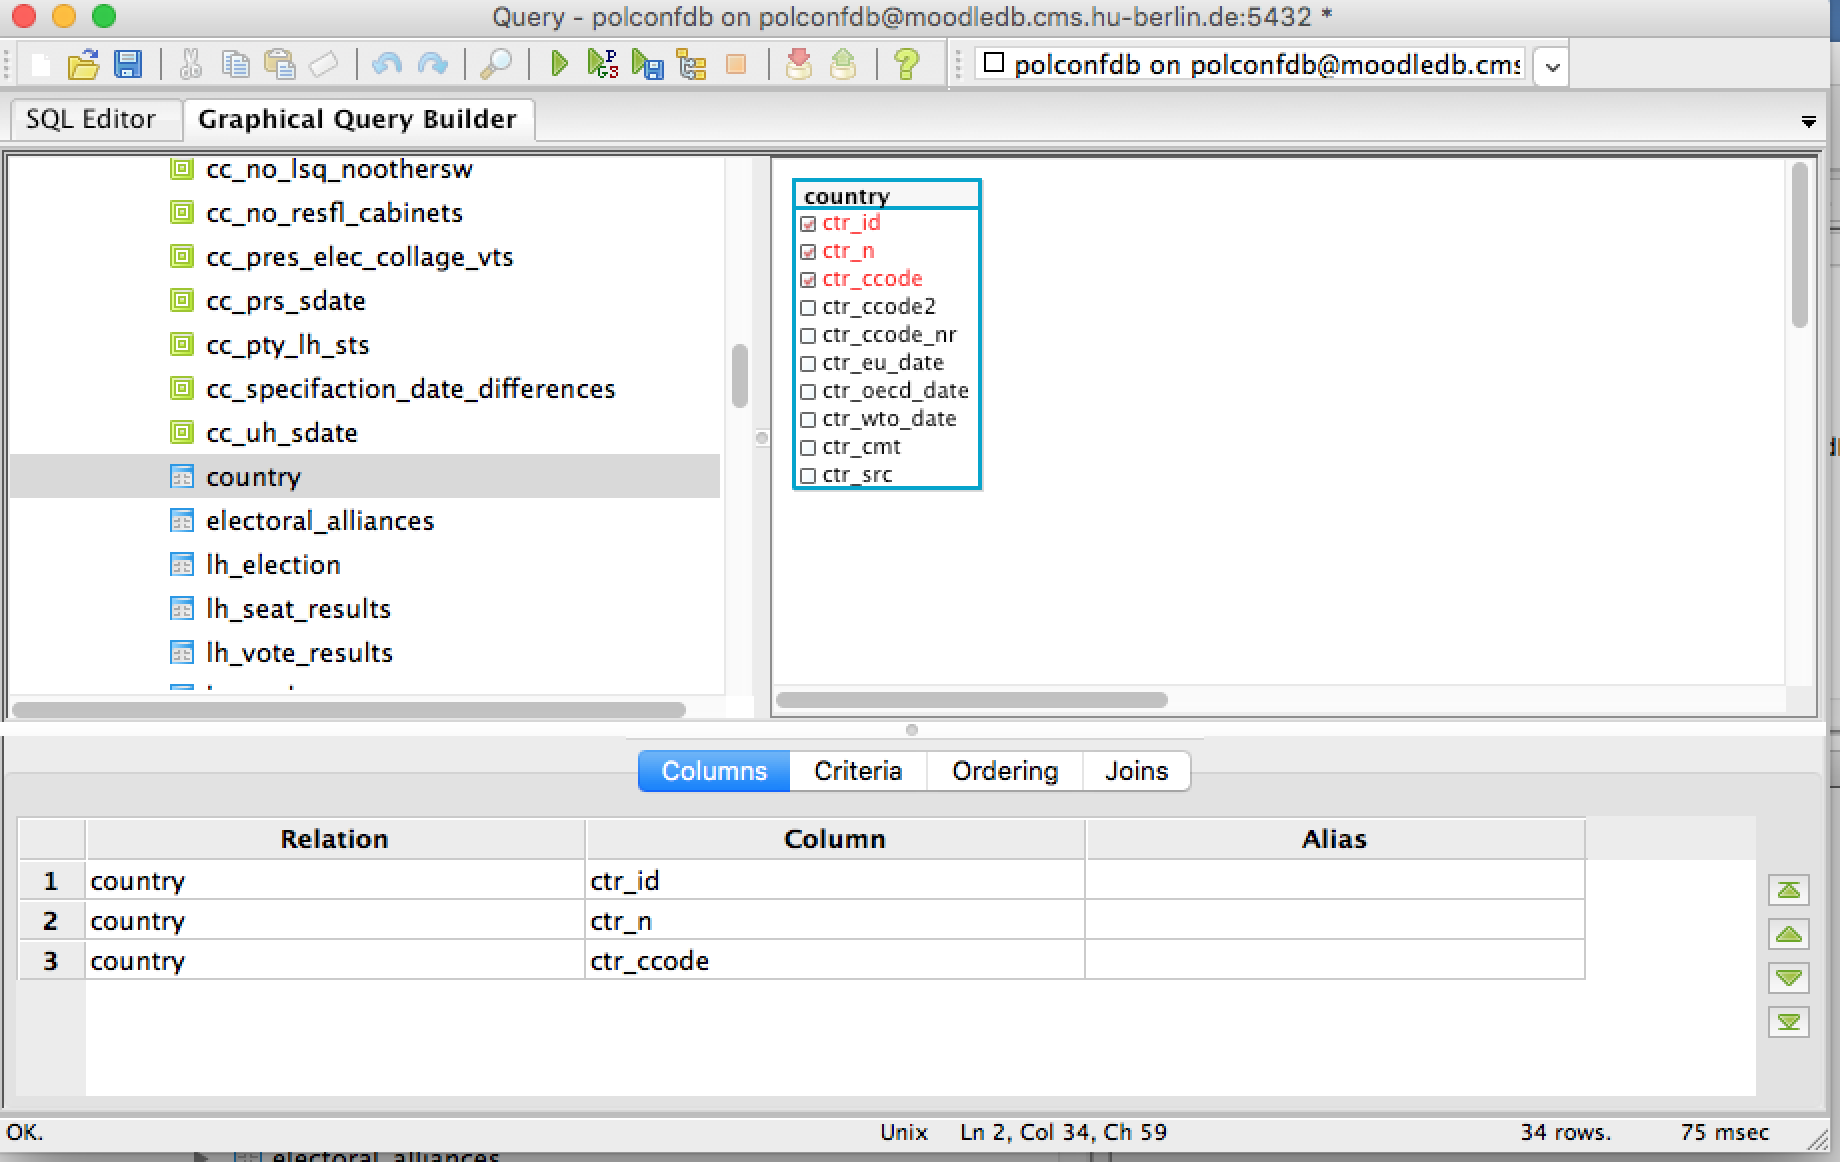
\includegraphics[width=\textwidth,trim= 0 0 0 0, clip]{pcdb_documentation_screenshots/pgadmin3_sql_query_tool_builder_country.png}
    \subcaption{Query data from country table  by manual selection in the `Graphical Query Builder' tab.}
    \label{fig_pgadmin3_sql_query_tool_builder_country}
  \end{subfigure} 
  \caption{Two ways to define queries in \texttt{pgadmin3}'s SQL-query tool window.}
\end{figure}

The double-clicking the green play-button in the SQL-query tool's toolbar (second from left in figure \ref{fig_pgadmin3_sql_query_tool_toolbar}) will execute the query; the result will be displayed as data table in the bottom panof the window.
The square shaped icon is the stop button (most right in figure \ref{fig_pgadmin3_sql_query_tool_toolbar}), which allows to cancel a running query.

\begin{figure}[ht!]
\centering
  
\includegraphics[width=.6\textwidth,trim= 0 0 0 0, clip]{pcdb_documentation_screenshots/pgadmin3_sql_query_tool_toolbar.png}
    \caption{Toolbar of \texttt{pgAdmin3}' SQL-query tool window.}
    \label{fig_pgadmin3_sql_query_tool_toolbar}
\end{figure}

The icon that combines a green play-button with a blue-shaded disc (third from right in figure \ref{fig_pgadmin3_sql_query_tool_toolbar}) will open the `Export data to file' wizard, which allows to write the result-set of a query to a file (see figure \ref{fig_pgadmin3_sql_query_tool_export_data_wizard}.
Select a column separator (default is a semicolon \texttt{;}), a quote character (default is the double qute \texttt{''}), select check-box `Column names' in case you want to include column (i.e., variable) names in the first row of the file, and select a path and file name to write to. Then click the `OK' button to export data to file.   

\begin{figure}[ht!]
\centering
  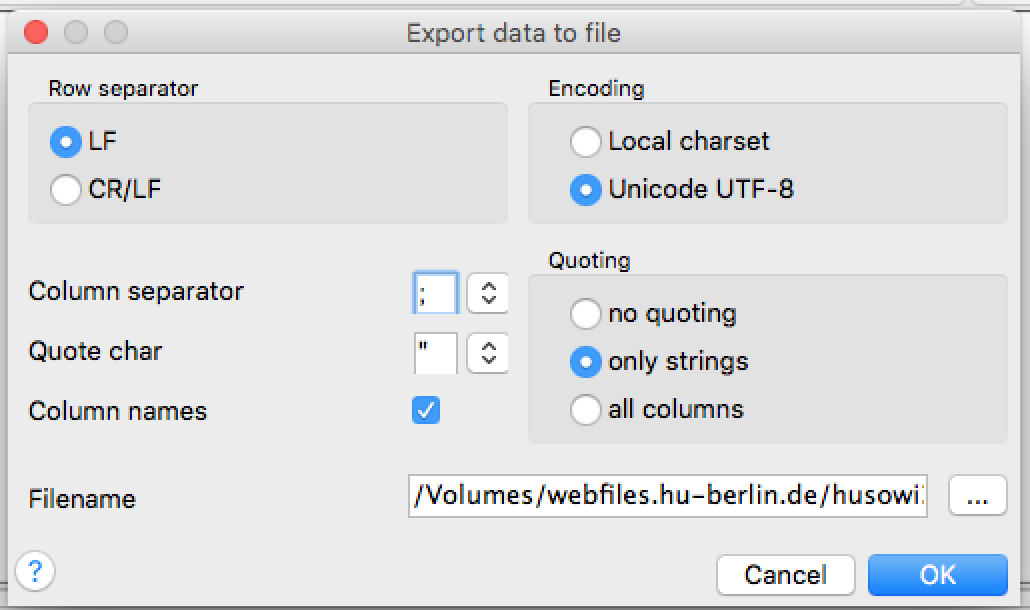
\includegraphics[width=.8\textwidth,trim= 0 0 0 0, clip]{pcdb_documentation_screenshots/pgadmin3_sql_query_tool_export_data_wizard.png}
    \caption{`Export data to file' wizard of \texttt{pgAdmin3}' SQL-query tool.}
    \label{fig_pgadmin3_sql_query_tool_export_data_wizard}
\end{figure}

When saving the result-set of the query to a file in the \texttt{.csv}-format, the result should look familiar to you. It's a plain semicolon-separated table (see figure \ref{fig_pgadmin3_sql_query_tool_export_data_result_example}).

\begin{figure}[ht!]
\centering
  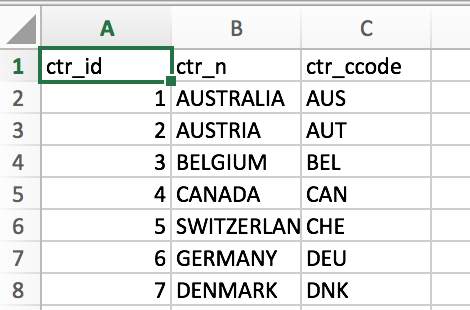
\includegraphics[width=.6\textwidth,trim= 0 0 0 0, clip]{pcdb_documentation_screenshots/pgadmin3_sql_query_tool_export_data_result_example.png}
    \caption{Result after exporting data with \texttt{pgAdmin3}'s `Export data to file' wizard.}
    \label{fig_pgadmin3_sql_query_tool_export_data_result_example}
\end{figure}




